%%%%%%%%%%%%%%%%%%%%%%%%%%%%%%%%%%%%%%%%%
% Beamer Presentation
% LaTeX Template
% Version 2.0 (March 8, 2022)
%
% This template originates from:
% https://www.LaTeXTemplates.com
%
% Author:
% Vel (vel@latextemplates.com)
%
% License:
% CC BY-NC-SA 4.0 (https://creativecommons.org/licenses/by-nc-sa/4.0/)
%
%%%%%%%%%%%%%%%%%%%%%%%%%%%%%%%%%%%%%%%%%

%----------------------------------------------------------------------------------------
%	PACKAGES AND OTHER DOCUMENT CONFIGURATIONS
%----------------------------------------------------------------------------------------

\documentclass[
	11pt, % Set the default font size, options include: 8pt, 9pt, 10pt, 11pt, 12pt, 14pt, 17pt, 20pt
	%t, % Uncomment to vertically align all slide content to the top of the slide, rather than the default centered
	%aspectratio=169, % Uncomment to set the aspect ratio to a 16:9 ratio which matches the aspect ratio of 1080p and 4K screens and projectors
]{beamer}


\usepackage{booktabs} % Allows the use of \toprule, \midrule and \bottomrule for better rules in tables
\usepackage{tikz}
\usepackage{colortbl}
\usepackage{array}
%----------------------------------------------------------------------------------------
%	SELECT LAYOUT THEME
%----------------------------------------------------------------------------------------

% Beamer comes with a number of default layout themes which change the colors and layouts of slides. Below is a list of all themes available, uncomment each in turn to see what they look like.

% \usetheme{default}
%\usetheme{AnnArbor}
%\usetheme{Antibes}
%\usetheme{Bergen}
% \usetheme{Berkeley}
%\usetheme{Berlin}
%\usetheme{Boadilla}
%\usetheme{CambridgeUS}
% \usetheme{Copenhagen}
%\usetheme{Darmstadt}
%\usetheme{Dresden}
%\usetheme{Frankfurt}
%\usetheme{Goettingen}
%\usetheme{Hannover}
%\usetheme{Ilmenau}
%\usetheme{JuanLesPins}
%\usetheme{Luebeck}
\usetheme{Madrid}
%\usetheme{Malmoe}
%\usetheme{Marburg}
%\usetheme{Montpellier}
% \usetheme{PaloAlto}
%\usetheme{Pittsburgh}
%\usetheme{Rochester}
% \usetheme{Singapore}
%\usetheme{Szeged}
%\usetheme{Warsaw}

%----------------------------------------------------------------------------------------
%	SELECT COLOR THEME
%----------------------------------------------------------------------------------------

% Beamer comes with a number of color themes that can be applied to any layout theme to change its colors. Uncomment each of these in turn to see how they change the colors of your selected layout theme.

% \usecolortheme{albatross}
%\usecolortheme{beaver}
%\usecolortheme{beetle}
%\usecolortheme{crane}
% \usecolortheme{dolphin}
%\usecolortheme{dove}
%\usecolortheme{fly}
%\usecolortheme{lily}
%\usecolortheme{monarca}
%\usecolortheme{seagull}
%\usecolortheme{seahorse}
%\usecolortheme{spruce}
%\usecolortheme{whale}
%\usecolortheme{wolverine}

%----------------------------------------------------------------------------------------
%	SELECT FONT THEME & FONTS
%----------------------------------------------------------------------------------------

% Beamer comes with several font themes to easily change the fonts used in various parts of the presentation. Review the comments beside each one to decide if you would like to use it. Note that additional options can be specified for several of these font themes, consult the beamer documentation for more information.

\usefonttheme{default} % Typeset using the default sans serif font
% \usefonttheme{serif} % Typeset using the default serif font (make sure a sans font isn't being set as the default font if you use this option!)
%\usefonttheme{structurebold} % Typeset important structure text (titles, headlines, footlines, sidebar, etc) in bold
%\usefonttheme{structureitalicserif} % Typeset important structure text (titles, headlines, footlines, sidebar, etc) in italic serif
%\usefonttheme{structuresmallcapsserif} % Typeset important structure text (titles, headlines, footlines, sidebar, etc) in small caps serif

%------------------------------------------------

%\usepackage{mathptmx} % Use the Times font for serif text
\usepackage{palatino} % Use the Palatino font for serif text

%\usepackage{helvet} % Use the Helvetica font for sans serif text
\usepackage[default]{opensans} % Use the Open Sans font for sans serif text
%\usepackage[default]{FiraSans} % Use the Fira Sans font for sans serif text
%\usepackage[default]{lato} % Use the Lato font for sans serif text

%----------------------------------------------------------------------------------------
%	SELECT INNER THEME
%----------------------------------------------------------------------------------------

% Inner themes change the styling of internal slide elements, for example: bullet points, blocks, bibliography entries, title pages, theorems, etc. Uncomment each theme in turn to see what changes it makes to your presentation.

\useinnertheme{default}
% \useinnertheme{circles}
% \useinnertheme{rectangles}
%\useinnertheme{rounded}
%\useinnertheme{inmargin}

%----------------------------------------------------------------------------------------
%	SELECT OUTER THEME
%----------------------------------------------------------------------------------------

% Outer themes change the overall layout of slides, such as: header and footer lines, sidebars and slide titles. Uncomment each theme in turn to see what changes it makes to your presentation.

\useoutertheme{default}
%\useoutertheme{infolines}
%\useoutertheme{miniframes}
%\useoutertheme{smoothbars}
%\useoutertheme{sidebar}
%\useoutertheme{split}
%\useoutertheme{shadow}
%\useoutertheme{tree}
%\useoutertheme{smoothtree}

%\setbeamertemplate{footline} % Uncomment this line to remove the footer line in all slides
%\setbeamertemplate{footline}[page number] % Uncomment this line to replace the footer line in all slides with a simple slide count

%\setbeamertemplate{navigation symbols}{} % Uncomment this line to remove the navigation symbols from the bottom of all slides

%----------------------------------------------------------------------------------------
%	PRESENTATION INFORMATION
%----------------------------------------------------------------------------------------

\title[Quantum Multi-string Matching]{Quantum Multi-string Matching} % The short title in the optional parameter appears at the bottom of every slide, the full title in the main parameter is only on the title page


\author[Allen Liu \and Kevin Tong]{Allen Liu \and Kevin Tong} % Presenter name(s), the optional parameter can contain a shortened version to appear on the bottom of every slide, while the main parameter will appear on the title slide

\institute[UW]{University of Waterloo} % Your institution, the optional parameter can be used for the institution shorthand and will appear on the bottom of every slide after author names, while the required parameter is used on the title slide and can include your email address or additional information on separate lines

\date[\today]{ECE 405C Winter 2025 \\ \today} % Presentation date or conference/meeting name, the optional parameter can contain a shortened version to appear on the bottom of every slide, while the required parameter value is output to the title slide

%----------------------------------------------------------------------------------------

\begin{document}

\newcommand*{\ket}[1]{\rvert#1\rangle}
%----------------------------------------------------------------------------------------
%	TITLE SLIDE
%----------------------------------------------------------------------------------------

\begin{frame}
    \titlepage % Output the title slide, automatically created using the text entered in the PRESENTATION INFORMATION block above
\end{frame}

%----------------------------------------------------------------------------------------
%	TABLE OF CONTENTS SLIDE
%----------------------------------------------------------------------------------------

% The table of contents outputs the sections and subsections that appear in your presentation, specified with the standard \section and \subsection commands. You may either display all sections and subsections on one slide with \tableofcontents, or display each section at a time on subsequent slides with \tableofcontents[pausesections]. The latter is useful if you want to step through each section and mention what you will discuss.

\begin{frame}
    \frametitle{Presentation Overview} % Slide title, remove this command for no title

    \tableofcontents % Output the table of contents (all sections on one slide)
    %\tableofcontents[pausesections] % Output the table of contents (break sections up across separate slides)
\end{frame}

%----------------------------------------------------------------------------------------
%	PRESENTATION BODY SLIDES
%----------------------------------------------------------------------------------------

\section{Problem Definition} % Sections are added in order to organize your presentation into discrete blocks, all sections and subsections are automatically output to the table of contents as an overview of the talk but NOT output in the presentation as separate slides

%------------------------------------------------

\begin{frame}
    \frametitle{String Matching}
    \begin{itemize}
        \item Text $S[0...n-1]$
        \item Pattern (or key) $P[0...m-1]$
        \item Strings from alphabet $\Sigma$
        \item Find set of indices $i$ such that $S[i..i+m] = P$
    \end{itemize}
    Example:
    \begin{itemize}
        \item $T$ = \texttt{"GTAT GATC TC"} (ignore spaces)
        \item $P_1$ = \texttt{"ATCT"}
        \item $P_2$ = \texttt{"TGAT"}
        \item $P_3$ = \texttt{"ACCC"}
        \item $P_1$ matches at 5, $P_2$ matches at 3, $P_3$ has no matches
    \end{itemize}
    \bigskip
    \begin{itemize}
        \item Multi-string matching: search $P_1, P_2, ...$ in $S$ simultaneously
    \end{itemize}
\end{frame}

%------------------------------------------------

\section{Classical Algorithms}
\subsection{Existing Algorithms}
\begin{frame}
    \frametitle{Classical Algorithms}
    \begin{itemize}
        \item Brute Force $\longrightarrow$ $O(mn)$
        \item Boyer-Moore $\longrightarrow$ $O(n+m)$, $O(mn)$ worst case
        \item Knuth-Morris-Pratt $\longrightarrow$ $O(n+m)$ worst case
        \item Suffix Tree/Array $\longrightarrow$ $O(m)/O(n\log n)$ + preproc
        \item Karp-Rabin - rolling hash $\longrightarrow$ $O(n+m)$ expected
    \end{itemize}

    \begin{center}

        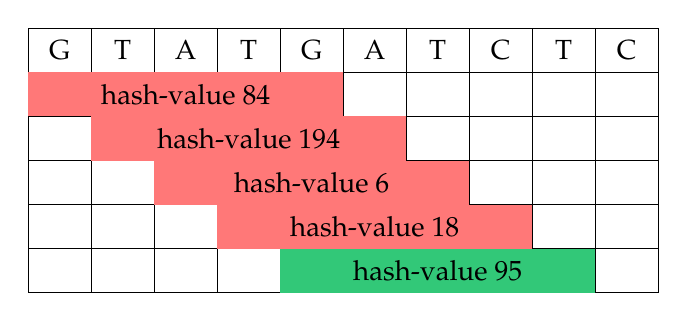
\begin{tikzpicture}[scale=0.8, y=0.7cm] % Scaling down the entire diagram with flatter cells
            % Define colors
            \definecolor{darkred}{RGB}{255,120,120}
            \definecolor{green}{RGB}{50,200,120}

            % Grid for cells with 6 rows
            \draw (0,0) -- (10,0);
            \draw (0,1) -- (10,1);
            \draw (0,2) -- (10,2);
            \draw (0,3) -- (10,3);
            \draw (0,4) -- (10,4);
            \draw (0,5) -- (10,5);
            \draw (0,6) -- (10,6);
            \draw (0,0) -- (0,6);
            \draw (1,0) -- (1,6);
            \draw (2,0) -- (2,6);
            \draw (3,0) -- (3,6);
            \draw (4,0) -- (4,6);
            \draw (5,0) -- (5,6);
            \draw (6,0) -- (6,6);
            \draw (7,0) -- (7,6);
            \draw (8,0) -- (8,6);
            \draw (9,0) -- (9,6);
            \draw (10,0) -- (10,6);

            % Add the letters at the top WITHOUT borders
            \foreach \x/\num in {0.5/G, 1.5/T, 2.5/A, 3.5/T, 4.5/G, 5.5/A, 6.5/T, 7.5/C, 8.5/T, 9.5/C} {
                    \node at (\x,5.5) {\num};
                }

            % Fill colors for different cells - one per row
            \fill[darkred] (0,4) rectangle (5,5); % First hash value
            \fill[darkred] (1,3) rectangle (6,4); % Second hash value 
            \fill[darkred] (2,2) rectangle (7,3); % Third hash value
            \fill[darkred] (3,1) rectangle (8,2); % Fourth hash value
            \fill[green] (4,0) rectangle (9,1); % Fifth hash value

            % Add the hash-value text
            \node at (2.5,4.5) {hash-value 84};
            \node at (3.5,3.5) {hash-value 194};
            \node at (4.5,2.5) {hash-value 6};
            \node at (5.5,1.5) {hash-value 18};
            \node at (6.5,0.5) {hash-value 95};

        \end{tikzpicture}

    \end{center}

    \begin{itemize}
        \item \alert{Polynomial Matching} $\longrightarrow$ $O(n\log n)$
    \end{itemize}
\end{frame}


%------------------------------------------------

\subsection{Polynomial Matching}
\begin{frame}
    \frametitle{Polynomial Matching}
    Calculate a fingerprint for $P$ and every $m$ character sequence in $S$; \alert {matching fingerprints} suggest pattern match!
    \bigskip
    \begin{align*}
        A & \mapsto -3 \\
        C & \mapsto 5  \\
        G & \mapsto -7 \\
        T & \mapsto 11
    \end{align*}
    \begin{align*}
        \texttt{"ATCT"}         & \longrightarrow \text{T}x^3 + \text{C}x^2 + \text{T}x + \text{A}   \\
                                & \longrightarrow  11x^3 + 5x^2 + 11x - 3                            \\
        \texttt{"GTAT GATC TC"} & \longrightarrow -7x^{15} + 11x^{14} - 3x^{13} + ... + 11x^7 + 5x^6
    \end{align*}
    Note that $P$ encoding is reversed (similar to convolution)
\end{frame}

%------------------------------------------------

\begin{frame}
    \frametitle{Polynomial Matching}
    Given polynomials
    \[
        P(x) = \sum_{i=0}^{m} a_i x^i, S(x) = \sum_{j=0}^{n} b_j x^j
    \]
    then
    \[
        R(x) = \sum_{k=0}^{m+n} c_k x^k
    \]
    where
    \[
        c_k = \sum_{i=0}^{k} a_i b_{k-i}, \quad \text{for } 0 \leq k \leq m+n,
    \]
    with the convention that \( a_i = 0 \) for \( i > m \) and \( b_j = 0 \) for \( j > n \).
\end{frame}

%------------------------------------------------

\begin{frame}
    \frametitle{Polynomial Matching}
    Coefficients of $R(x)$ correspond to ``dot products'' between substrings.
    \begin{align*}
        P(x) & = 11x^3 + 5x^2 + 11x - 3                                    \\
        S(x) & = -7x^{15} + 11x^{14} - 3x^{13} + ... + 11x^7 + 5x^6        \\
        R(x) & = ... + 71x^8 + 0x^9 + 276x^{10} + 98x^{11} - 4x^{12} + ...
    \end{align*}
    Degrees map to index:
    \begin{align*}
        15 & \text{ yields index } 0 \\
        14 & \text{ yields index } 1 \\
           & \hspace{0.8cm}...       \\
        11 & \text{ yields index } 4 \\
        10 & \text{ yields index } 5 \\
        9  & \text{ yields index } 6 \\
    \end{align*}
\end{frame}

%------------------------------------------------

\begin{frame}
    \frametitle{Polynomial Matching}
    Coefficients of $R(x)$ correspond to ``dot products'' between substrings.
    \begin{align*}
        P(x) & = 11x^3 + 5x^2 + 11x - 3                                    \\
        S(x) & = -7x^{15} + 11x^{14} - 3x^{13} + ... + 11x^7 + 5x^6        \\
        R(x) & = ... + 71x^8 + 0x^9 + 276x^{10} + 98x^{11} - 4x^{12} + ...
    \end{align*}
    Notice that $\|P\|^2 = 11^2 + 5^2 + 11^2 + (-3)^2 = 276$ \\
    \bigskip
    We get exact fingerprint match for single patterns. Let's extend to multiple patterns...
\end{frame}


%------------------------------------------------

\begin{frame}
    \frametitle{Polynomial Matching}
    Add patterns together:
    \begin{align*}
        P(x) & = P_1(x) + P_2(x)                                                        \\
        S(x) & = -7x^{15} + 11x^{14} - 3x^{13} + ... + 11x^7 + 5x^6                     \\
        R(x) & = ... + 94x^8 + 240x^9 + 272x^{10} + 64x^{11} + 296x^{12} - 60x^{13} ...
    \end{align*}
    \bigskip
    No more exact matches, but higher values = likelier index.
\end{frame}

%------------------------------------------------

\subsection{Polynomial Multiplication}

\begin{frame}
    \frametitle{Polynomial Multiplication}
    Multiple algorithms:
    \begin{itemize}
        \item Naïve polynomial multiplication $\longrightarrow$ $O(n^2)$
        \item Karatsuba Algorithm $\longrightarrow$ $O(n^{\log_3 2}) = O(n^{1.59})$
        \item FFT $\longrightarrow$ $O(n\log n)$
    \end{itemize}
\end{frame}

%------------------------------------------------


\begin{frame}
    \frametitle{Point Value Form}
    \begin{theorem}[Lagrange Interpolation]
        For any $n$ points $(x_i, y_i) \in \mathbb R^2$ with no two $x_i$ the same, there exists a unique polynomial $A(x)$ of degree at most $n-1$ that interpolates these points.
    \end{theorem}
    Given polynomials $A(x)$ and $B(x)$ of degree $n$, we can represent them as
    \begin{align*}
        A & : \{(x_0, A(x_0)), (x_1, A(x_1)),\dots , (x_{n-1}, A(x_{n-1})) \} \\
        B & : \{(x_0, B(x_0)), (x_1, B(x_1)),\dots , (x_{n-1}, B(x_{n-1})) \}
    \end{align*}
    Then their product $C(x) = A(x)B(x)$ is
    \[
        C: \{(x_0, A(x_0)B(x_0)), (x_1, A(x_1)B(x_1)),\dots , (x_n, A(x_{n-1})B(x_{n-1})) \}
    \]
\end{frame}


%------------------------------------------------


\begin{frame}
    \frametitle{Polynomial Multiplication}
    Algorithm idea:
    \begin{enumerate}
        \item Evaluate $A(x)$ and $B(x)$ at $n$ points
              \begin{itemize}
                  \item $O(n)$ multiplications per point
                  \item $O(n)$ points
                  \item $O(n^2)$ overall, no speedup
              \end{itemize}
        \item Multiply element-wise
        \item Interpolate to find $C(x)$ coefficients
    \end{enumerate}
    \bigskip
    But this works for any $n$ inputs. What if we try the $n^{th}$ roots of unity?
    \begin{align*}
        \hat{a}_k = A(\omega_n^k) & = \sum_{j=0}^n a_j e^{\frac{2\pi ijk}{n}}
    \end{align*}
    for $0 \leq k \leq n-1$. This is \alert{DFT}!
\end{frame}

%------------------------------------------------

\begin{frame}
    \frametitle{Polynomial Multiplication with FFT}
    \begin{enumerate}
        \item Apply FFT to the coefficients of $A(x)$ and $B(x)$ \\
              With $\vec{a} = [a_0\,\,a_1\dots a_{n-1}]^T$ and $\vec{b} = [b_0\,\,b_1\dots b_{n-1}]^T$, then
              \begin{align*}
                  \vec{\alpha} & = \text{FFT}(\vec{a}) \tag*{$O(n\log n)$} \\
                  \vec{\beta}  & = \text{FFT}(\vec{b}) \tag*{$O(n\log n)$}
              \end{align*}
        \item Perform the Hadamard (element-wise) product of coefficients
              \begin{align*}
                  \vec{\gamma} & = \vec{\alpha} \odot \vec{\beta}                                                       \\
                               & = [\alpha_0\beta_0\,\,\,\,\alpha_1\beta_1\dots\alpha_{n-1}\beta_{n-1}]^T \tag*{$O(n)$}
              \end{align*}
        \item Apply Inverse FFT
              \begin{align*}
                  \vec{c} & = \text{IFFT}(\vec{\gamma}) \tag*{$O(n\log n)$}
              \end{align*}
    \end{enumerate}
\end{frame}

%------------------------------------------------

% \begin{frame}
%     \frametitle{Polynomial Multiplication with QFT}
%     \begin{enumerate}
%         \item Apply QFT to quantum states $\ket{\psi}$ and $\ket{\phi}$ 
%         that are amplitude encodings of polynomial cofficients \\
%         \item Perform the Hadamard (element-wise) product of 
%             $\text{QFT}(\ket{\psi})$ and $\text{QFT}(\ket{\phi})$
%         \item Apply Inverse QFT
%     \end{enumerate}
% \end{frame}

%------------------------------------------------

\section{Quantum Algorithms}
\subsection{Polynomial Multiplication with QFT}
\begin{frame}
    \frametitle{Polynomial Multiplication with QFT}
    \begin{center}
        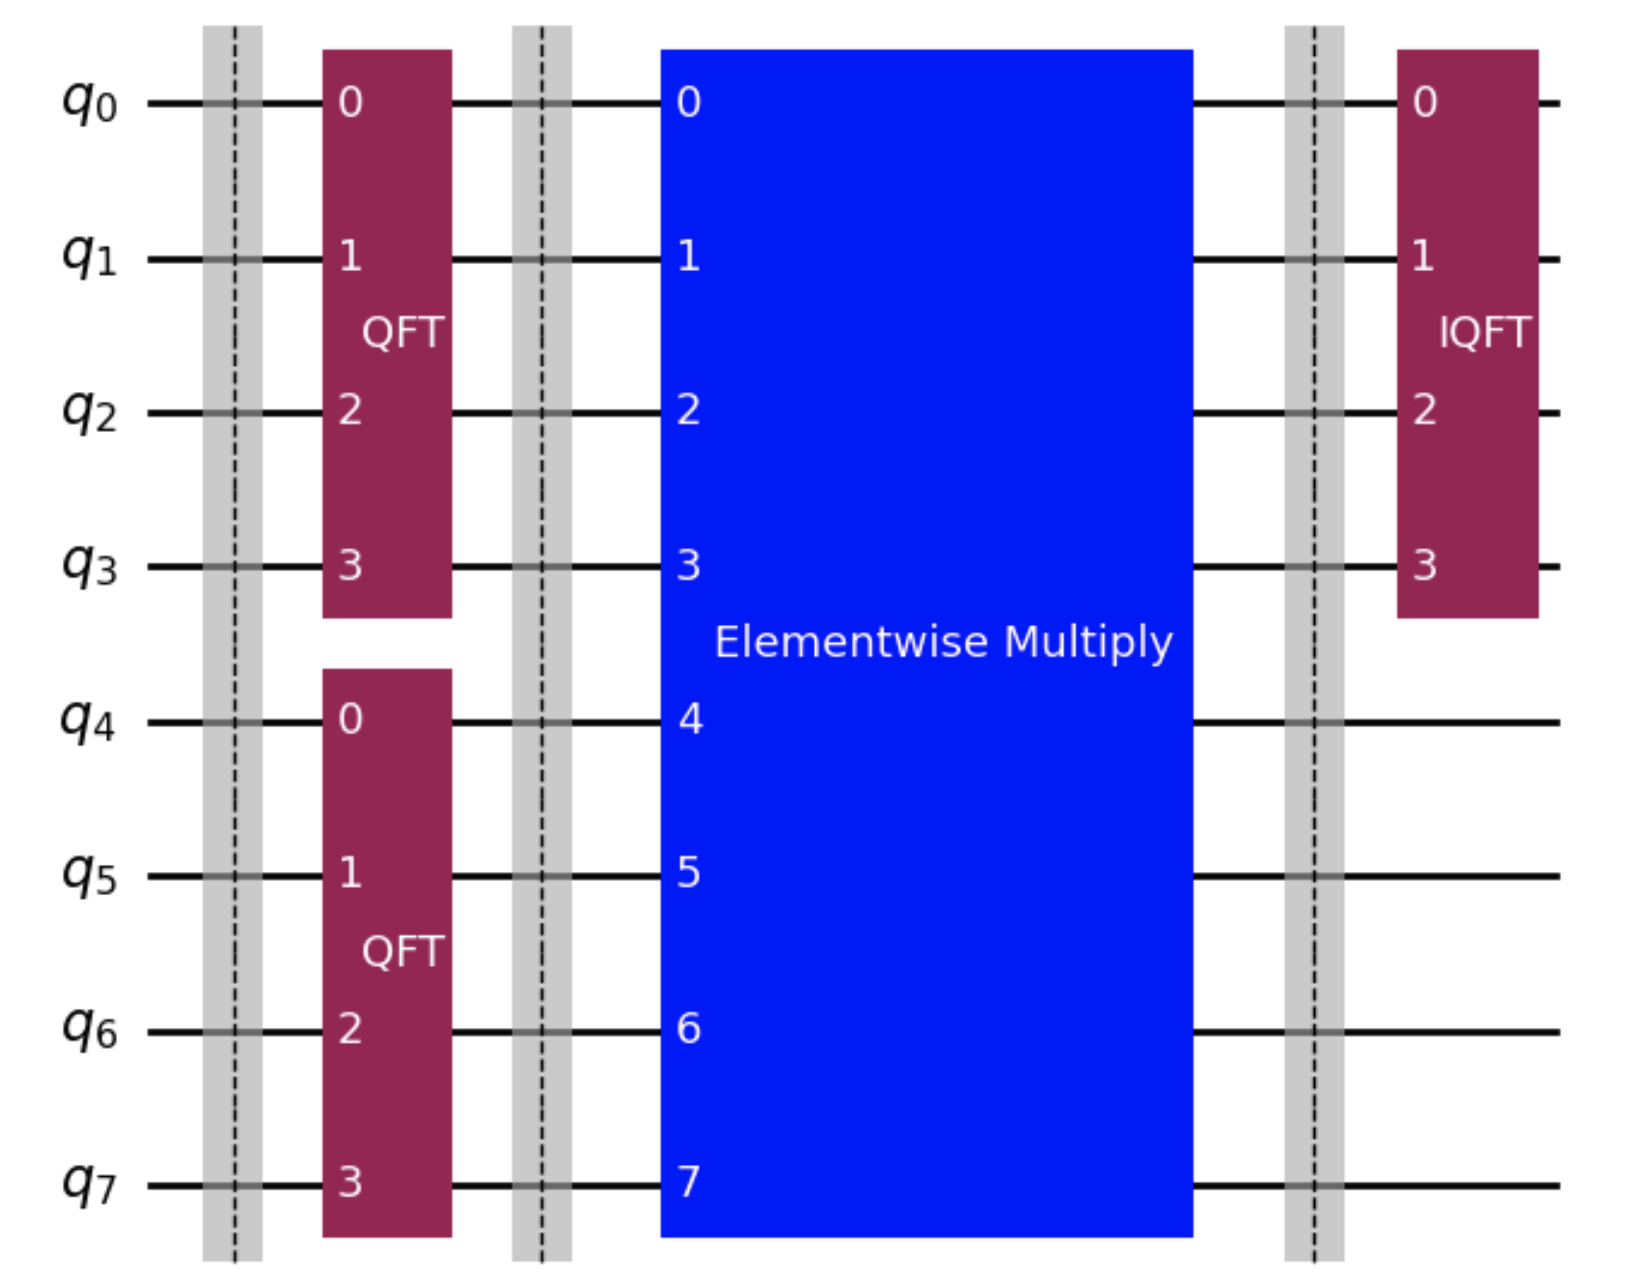
\includegraphics[scale=0.28]{unitary.png}
    \end{center}
    Polynomial multiplication for degree up to $n=2^4 - 1 = 15$
\end{frame}

%------------------------------------------------

\subsection{Elementwise Multiply}
\begin{frame}
    \frametitle{Elementwise Multiply}
    Is there such a unitary operator? Define
    \begin{align*}
        \ket{\alpha}             & = \alpha_0\ket{00} + \alpha_1\ket{01} + \alpha_2\ket{10} + \alpha_3\ket{11}                                           \\
        \ket{\beta}              & = \beta_0\ket{00} + \beta_1\ket{01} + \beta_2\ket{10} + \beta_3\ket{11}                                               \\
        \ket{\alpha \odot \beta} & = C\left(\alpha_0\beta_0\ket{00} + \alpha_1\beta_1\ket{01} + \alpha_2\beta_2\ket{10} + \alpha_3\beta_3\ket{11}\right)
    \end{align*}
    for some normalization constant $C$
    \[
        U\ket{x}\ket{y} = U\ket{x}\ket{x \odot y}
    \]
    If $\ket{y} = \frac{1}{2} \left(\ket{00} + \ket{01} + \ket{10} + \ket{11}\right)$ $\longrightarrow$ violates \alert{no-cloning theorem}
\end{frame}

%------------------------------------------------

\begin{frame}
    \frametitle{Elementwise Multiply}
    Allow probabilistic operator:
    \begin{align*}
        \ket{\alpha}\ket{\beta} & = \alpha_0\beta_0 \ket{0000} + \alpha_0\beta_1\ket{0001} + \dots               \\
                                & \hspace{0.45cm} \alpha_1\beta_0\ket{0100} + \alpha_1\beta{1}\ket{0101} + \dots \\
                                & \hspace{0.45cm} \dots + \alpha_2\beta_2\ket{1010} + \dots                      \\
                                & \hspace{0.45cm} \dots + \alpha_3\beta_3\ket{1111} + \dots
    \end{align*}
    Want when \textcolor{red}{first two bits} = \textcolor{blue}{last two bits}.\\
    \bigskip
    Use CNOT to test for equality.
\end{frame}

%------------------------------------------------

\begin{frame}
    \frametitle{Elementwise Multiply}
    \begin{center}
        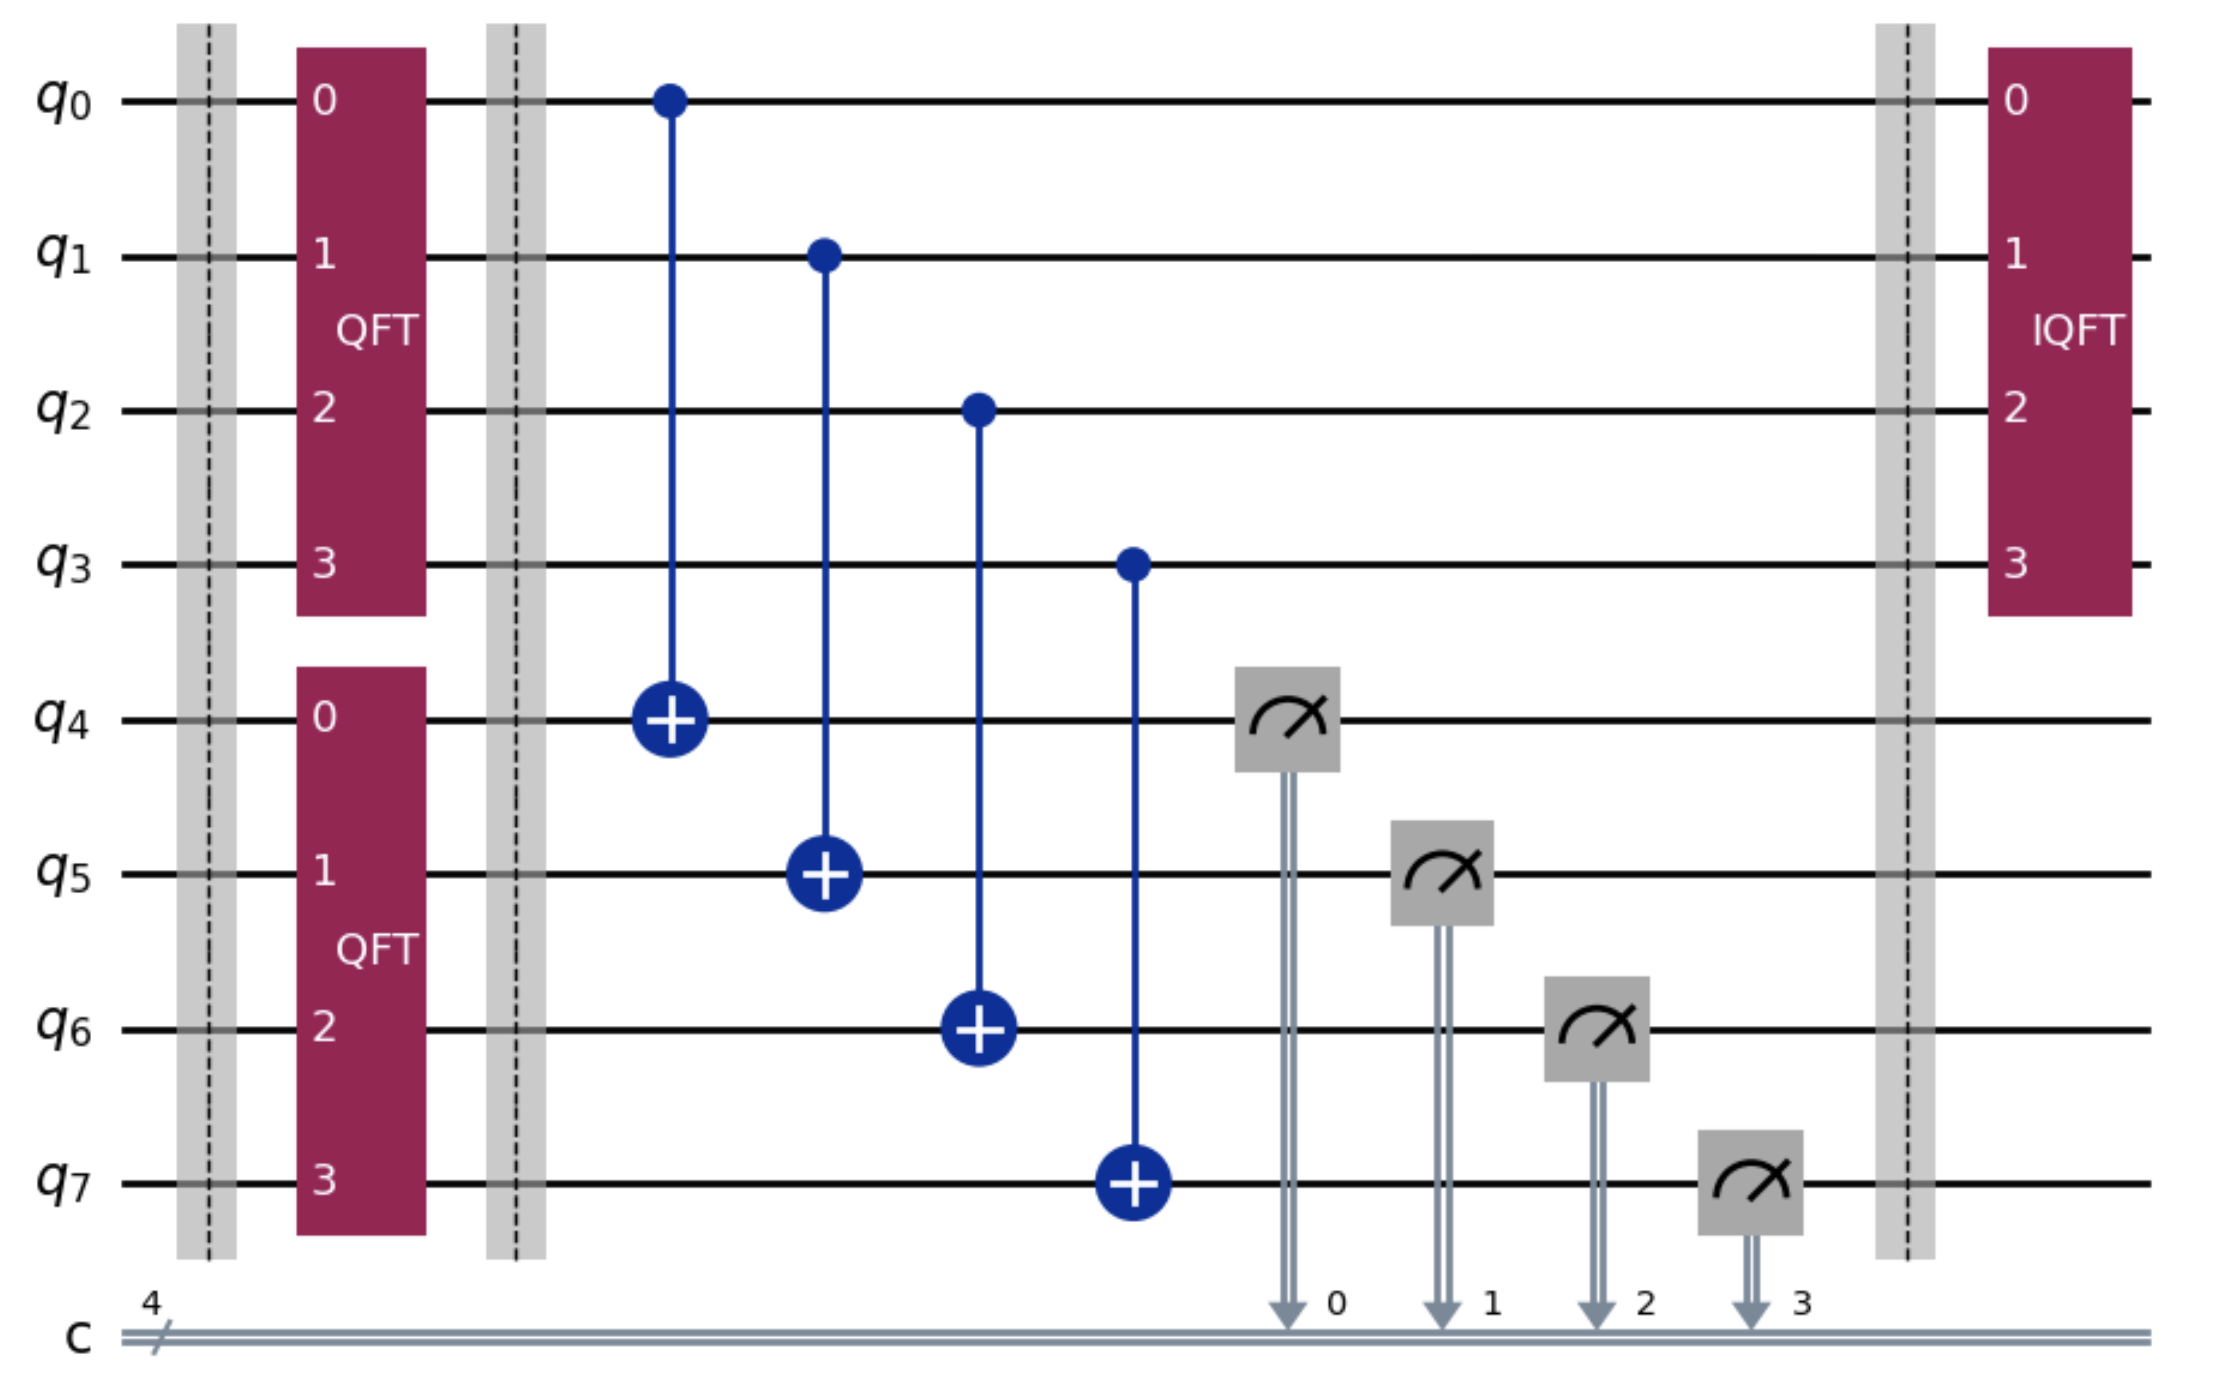
\includegraphics[scale=0.28]{elementwise.png}
    \end{center}
\end{frame}


%------------------------------------------------

\begin{frame}
    \frametitle{Elementwise Multiply}
    \begin{align*}
        \ket{\alpha}\ket{\beta}                                        & = \alpha_0\beta_0 \ket{\alert{0000}} + \alpha_0\beta_1\ket{0001} + \dots               \\
                                                                       & \hspace{0.45cm} \alpha_1\beta_0\ket{0100} + \alpha_1\beta{1}\ket{\alert{0101}} + \dots \\
                                                                       & \hspace{0.45cm} \dots + \alpha_2\beta_2\ket{\alert{1010}} + \dots                      \\
                                                                       & \hspace{0.45cm} \dots + \alpha_3\beta_3\ket{\alert{1111}} + \dots                      \\\\
        \text{CNOT}_{0, 2}\text{CNOT}_{1, 3} \;\ket{\alpha}\ket{\beta} & = \alpha_0\beta_0 \ket{\alert{0000}} + \alpha_0\beta_1\ket{0001} + \dots               \\
                                                                       & \hspace{0.45cm} \alpha_1\beta_0\ket{0101} + \alpha_1\beta{1}\ket{\alert{0100}} + \dots \\
                                                                       & \hspace{0.45cm} \dots + \alpha_2\beta_2\ket{\alert{1000}} + \dots                      \\
                                                                       & \hspace{0.45cm} \dots + \alpha_3\beta_3\ket{\alert{1100}} + \dots                      \\
    \end{align*}
    Measure the last two qubits, success when $\ket{00}$ $\longrightarrow$ elementwise multiply in first two qubits!
\end{frame}

%------------------------------------------------

% \begin{frame}
%     \frametitle{Using Measurement for Validity}
%     To ensure the validity of quantum element-wise multiplication,
%     we require the last qubits to be measured as all zero.
%     \newline\newline
%     Consider the simplest case: the element-wise product of two qubits' states
%     \begin{align*}
%          & CNOT_{1\to 2}((a_0\ket{0} + a_1\ket{1}) \otimes (b_0\ket{0} + b_1\ket{1}))         \\
%          & = CNOT_{1\to 2}(a_0b_0\ket{00} + a_0b_1\ket{01} + a_1b_0\ket{10} + a_1b_1\ket{11}) \\
%          & = a_0b_0\ket{00} + a_0b_1\ket{01} + a_1b_0\ket{11} + a_1b_1\ket{10}                \\
%     \end{align*}
%     Note how the $a_0b_0$ and $a_1b_1$ products are only associated with terms where the second qubit is $\ket{0}$,
%     and a coefficient product can be ``chosen'' using the state of the first qubit.
% \end{frame}

%------------------------------------------------
\subsection{Analysis \& Results}
\begin{frame}
    \frametitle{Algorithmic Analysis}
    Let $N = \log_2 n$ be the number of qubits needed to represent the polynomial 
    produced by multiplying $A(x)$ and $B(x)$.

    \bigskip
    Each QFT: \textcolor{blue}{$O(N^2)$ gates}.

    \bigskip
    Element-wise multiplication: \textcolor{blue}{$O(N)$ CNOT gates}, 
    but requries an expected $O(n)$ measurements for a result where 
    the last $N$ qubits are all zero.

    \bigskip
    So the total cost is $O(\log^2 n)$ gates, but expected $O(n)$ shots per successful sample.
\end{frame}

%------------------------------------------------

\begin{frame}
    \frametitle{Qiskit Results}
    Text: \texttt{"GTAT GATC TC"}
    Key: \texttt{"ATCT"}

    \begin{center}
        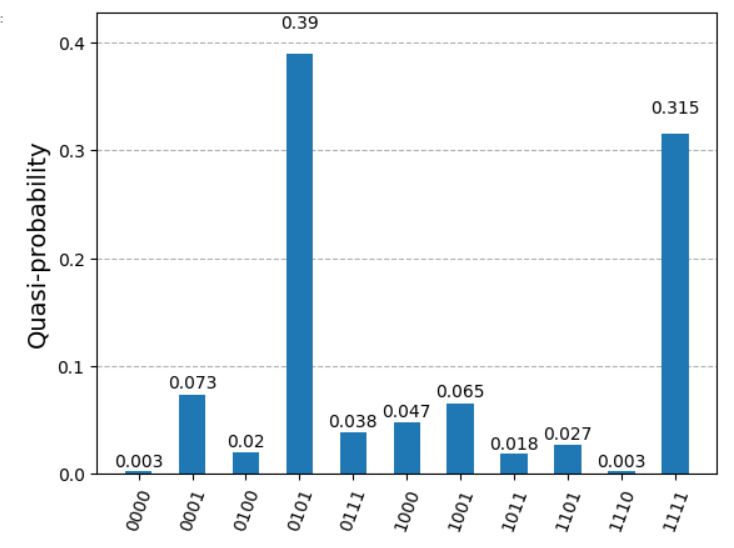
\includegraphics[scale=0.5]{aer_search.png}
    \end{center}
    Notice that the highest quasi-probability is for state $1010_2$! 
\end{frame}

%------------------------------------------------

\begin{frame}
    \frametitle{Multi-String Matching}
    \begin{itemize}
        \item Text: \texttt{"GTAT GATC TC"}
        \item Key 1: \texttt{"ATCT"}
        \item Key 2: \texttt{"TGAT"}
        \item Key 3: \texttt{"ACCC"}
    \end{itemize}

    \begin{center}
        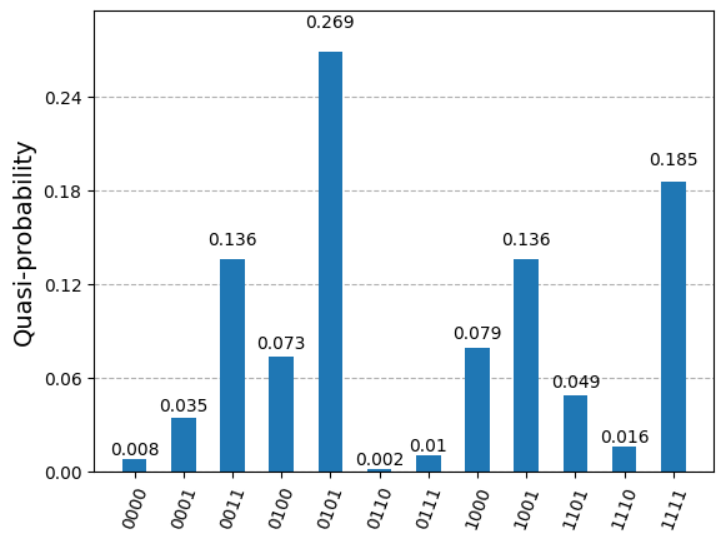
\includegraphics[scale=0.5]{aer_multi_string_match.png}
    \end{center}
\end{frame}

%------------------------------------------------

\begin{frame}
    \frametitle{More Qiskit Results}
    \begin{itemize}
        \item Text: 90 randomly generated characters $\in \{A,T,C,G\}$
        \item Key: 52 characters
    \end{itemize}

    \begin{center}
        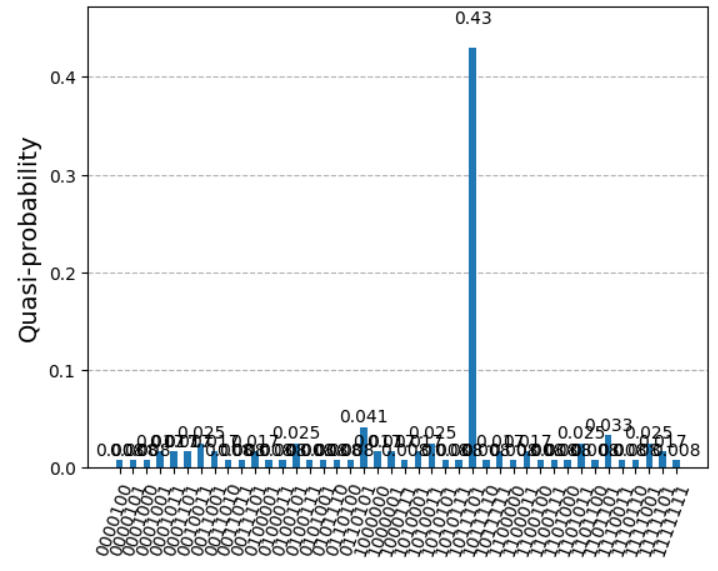
\includegraphics[scale=0.5]{aer_stress_test.png}
    \end{center}
\end{frame}

%------------------------------------------------

\section{Next Steps}
\begin{frame}
    \frametitle{Next Steps}
    \begin{enumerate}
        \item Sometimes patterns destructively interfere $\longrightarrow$ better combination method than addition?
        \item Encoding uses primes $\longrightarrow$ better interference patterns?
        \item Wasteful elementwise multiply $\longrightarrow$ reconstruct data using shifted multiply?
        
        \bigskip
        E.g. measure $\ket{01}$:
        \[
            \ket{\psi} = \alpha_0\beta_1 \ket{0001} + \alpha_1\beta_0 \ket{0101} + \alpha_2\beta_3 \ket{1001} + \alpha_3\beta_2 \ket{1101}
        \]
    \end{enumerate}
\end{frame}

%------------------------------------------------

\begin{frame} % Use [allowframebreaks] to allow automatic splitting across slides if the content is too long
    \frametitle{References}

    \begin{thebibliography}{99} % Beamer does not support BibTeX so references must be inserted manually as below, you may need to use multiple columns and/or reduce the font size further if you have many references
        \footnotesize % Reduce the font size in the bibliography

        \bibitem[Cooley \& Tukey]{p1}
        James W. Cooley, John W. Tukey (1965)
        \newblock An Algorithm for the Machine Calculation of Complex Fourier Series
        \newblock \emph{https://www.ams.org/journals/mcom/1965-19-090/S0025-5718-1965-0178586-1/S0025-5718-1965-0178586-1.pdf}

        \bibitem[Richard M. Karp \& Michael O. Rabin]{p2}
        Richard M. Karp \& Michael O. Rabin (1987)
        \newblock Efficient Randomized Pattern-matching Algorithms
        \newblock \emph{https://doi.org/10.1147/rd.312.0249}

        \bibitem[Ramezani et. al., 2023]{p3}
        Mehdi Ramezani, Morteza Nikaeen, Farnaz Farman, Seyed Mahmoud Ashrafi and Alireza Bahrampour (2023)
        \newblock Quantum Multiplication Algorithm Based on the Convolution Theorem
        \newblock \emph{https://arxiv.org/pdf/2306.08473}

    \end{thebibliography}
\end{frame}


\end{document}